\UNsection{1.3 - Extension \& Uniqueness}
\seteqgroup{3}

This entire section is entirely a pursuit of proving the following theorem:\\[5pt]

\textbf{Theorem 3.1: } A probability measure on a field has a unique extension to the generated $\sigma$-field\\[5pt]  

In other words, let $P$ be a probability measure on a field $\mathbb{F}_0$ of subsets of $\Omega$, and let $\mathcal{F}=\sigma(\mathcal{F}_0)$. Then there exists a probability measure $Q$ on $\mathcal{F}$ such that $Q(A)=P(A)$ for $A\in \mathcal{F}_0$. Further, if $Q'$ is another probability measure on $\mathcal{F}$ such that $Q'(A)=P(A)$ for $A\in \mathcal{F}_0$, then $Q'(A)=Q(A)$ for $A \in \mathcal{F}$\\[5pt]

\UNsubsection{Extension - Carathéodory’s Method} \quad

    Let $P$ be a probability measure on a field $\mathcal{F}_0$. We want to extend $P$ to a more general class. For each subset $A$ of $\Omega$, we define its \textbf{Outer Measure} as the following:
    \begin{UNequation}
        P^{\medstar}(A)=\textbf{inf}\sum_n P(A_n) \quad \quad \scalebox{0.8}[0.8]{\textbf{Outer Measure}}
    \end{UNequation}

    Where the infimum extends over all finite and infinite sequences $A_1,A_2,...$ of $\mathcal{F}_0$-sets satisfying $A \subset \bigcup_n A_n$. When considered together, the $A_n$ form a good covering of $A$ if they do not overlap very much, nor do they extend very far beyond $A$. When this is this case $\sum_n P(A_n)$ is a good outer approximation of the measure $A$. As a result of this, (3.1) acts as our initial attempt to assign a measure to A.

    Conversely, the \textbf{Inner Measure} approximates $A$ from the inside by subtracting the compliment of $A$ from one:
    \begin{UNequation}
        P_{\medstar}(A)=1- P^{\medstar}(A^c) \quad \quad \scalebox{0.8}[0.8]{\textbf{Inner Measure}}
    \end{UNequation}

    Using these two pre-measures, we want to assign measure to those A that satisfy the following condition:
    \begin{UNequation}
        P^{\medstar}(A\cap E)+ P^{\medstar}(A^c \cap E)= P^{\medstar}(E) \quad \text{for every set }  E
    \end{UNequation}

    A set $A$ is called \textbf{\boldmath\( P^{\medstar}\textbf{-Measurable} \)} if (3.3) holds for all $E$.
    Let $\mathcal{M}$ be the class of $P^{\medstar}$-measurable sets. Our task then becomes to show that:
    \begin{enumerate}[topsep=0pt, itemsep=-3pt]
        \item[] $\mathcal{M}$ contains $\sigma(\mathcal{F}_0)$ and  
        \item[] The restriction of $P^{\medstar}$ to $\sigma(\mathcal{F}_0)$ is the required extension of $P$
    \end{enumerate}
    We accomplish this by employing four key properties of the set-function $P^{\medstar}$:
     \begin{enumerate}[label=\textbf{\roman*.}, topsep=0pt, itemsep=-3pt]
        \item $P^{\medstar}(\emptyset)=0$
        \item $P^{\medstar}$ is non-negative: $P^{\medstar} \geq 0$ for every $A \subset \Omega$
        \item $P^{\medstar}$ is monotone: $A \subset B$ implies $P^{\medstar}(A) \leq P^{\medstar}(B)$
        \item $P^{\medstar}$ is countably subadditive: $P^{\medstar}(\bigcup_n A_n) \leq \sum_n P^{\medstar}(A_n)$
     \end{enumerate}

     The first three of these properties are true by definition.

    \textbf{Proof of iv.}
    \vspace{-1ex}
    \begin{proofline}
        For a given $ \varepsilon $, choose $\mathcal{F}_0$-sets $B_{nk}$ such that $A_n \subseteq \bigcup_k B_{nk}$ and $\sum_k P(B_{nk}) < P^{\medstar}(A_n) + \varepsilon / 2^n$, which is possible by the definition (3.1). Now $\bigcup_n A_n \subseteq \bigcup_{n,k} B_{nk}$, so that $P^{\medstar}(\bigcup_n A_n) < \sum_{n,k} P(B_{nk}) < \sum_n \left( P^{\medstar}(A_n) + \varepsilon / 2^n \right)$, and \textbf{iv} follows. \hfill \qed.
    \end{proofline}

    $A$ lies in the class $\mathcal{M}$ of $P^{\medstar}$-measurable sets if it splits each $E$ in $2^{\omega}$ in such a way that $P^{\medstar}$ adds for the pieces; mathematically that is:
    \begin{UNequation}
    \begin{aligned}
    &P^{\medstar}(A \cap E) + P^{\medstar}(A^c \cap E) \leq P^{\medstar}(E)\\
    &\scalebox{0.8}[0.8]{$\elbowarrow \text{i.e., } A \text{ splits } E \text{ in a way that preserves the additivity of } P^{\medstar}$}    
    \end{aligned}
    \end{UNequation}

    \needspace{8\baselineskip}
    \textbf{Lemma 1: } The class $\mathcal{M}$ is a field.

    \textbf{Proof: }
    \vspace{-1ex}
    \begin{proofline}
        It is clear that \( \Omega \in \mathcal{F}' \) and that \( \mathcal{F}' \) is closed under complementation. Suppose that \( A, B \in \mathcal{F}' \) and \( E \subseteq \Omega \). Then
        \begin{UNequation}
        \scalebox{0.8}[0.8]{$\begin{aligned}
        P^{\medstar}(E) &= P^{\medstar}(B \cap E) + P^{\medstar}(B^c \cap E) \\
               &= P^{\medstar}(A \cap B \cap E) + P^{\medstar}(A^c \cap B \cap E) \\
               &\quad + P^{\medstar}(A \cap B^c \cap E) + P^{\medstar}(A^c \cap B^c \cap E) \\
               &\geq P^{\medstar}(A \cap B \cap E) \quad (\text{by subadditivity})\\
               &\quad + P^{\medstar}\big( (A^c \cap B \cap E) \cup (A \cap B^c \cap E) \cup (A^c \cap B^c \cap E) \big) \\
               &= P^{\medstar}((A \cap B) \cap E) + P^{\medstar}((A \cap B)^c \cap E),
        \end{aligned}$}
        \end{UNequation}
        
        \vspace{-4ex}
        
        Hence \( A \cap B \in \mathcal{F}' \), and \( \mathcal{F}' \) is a field. \hfill \qed
    \end{proofline}

    \needspace{8\baselineskip}
    \textbf{Lemma 2: } If $A_1, A_2, ...$ is a finite sequence or infinite sequence of $\mathcal{M}$-sets, then for each:$E\subset \Omega$
    \begin{UNequation}
        P^{\medstar}\left(E\cap\left(\bigcup_k A_k \right) \right) = \sum_k P^{\medstar}(E\cap A_k) 
    \end{UNequation}

    \needspace{10ex}
    \textbf{Proof: }
    \vspace{-1ex}
    \begin{proofline}
        Consider first the case of finitely many \( A_k \), say \( n \) of them. For \( n = 1 \), there is nothing to prove. In the case \( n = 2 \), if \( A_1 \cup A_2 = \Omega \), then (3.6) is just (3.4) with \( A_1 \) (or \( A_2 \)) in the role of \( A \). If \( A_1 \cup A_2 \subsetneq \Omega \), split \( E \cap (A_1 \cup A_2) \) by \( A_1 \) and \( A_2 \) (or by \( A_2 \) and \( A_1 \)) and use (3.4) and disjointness.

        Assume (3.6) holds for the case of \( n - 1 \) sets. By the case \( n = 2 \), together with the induction hypothesis,
        \[
        P^{\medstar}\left( E \cap \bigcup_{k=1}^n A_k \right)
        = P^{\medstar}\left( E \cap \bigcup_{k=1}^{n-1} A_k \right) + P^{\medstar}(E \cap A_n)
        = \sum_{k=1}^n P^{\medstar}(E \cap A_k).
        \]
        Thus, (3.6) holds in the finite case.
        
        For the infinite case, use monotonicity:
        \[
        P^{\medstar}\left( E \cap \bigcup_{k=1}^\infty A_k \right)
        = \lim_{n \to \infty} P^{\medstar}\left( E \cap \bigcup_{k=1}^n A_k \right)
        = \lim_{n \to \infty} \sum_{k=1}^n P^{\medstar}(E \cap A_k).
        \]
        Hence, the left side of (3.6) is greater than or equal to the right.
        The reverse inequality follows by countable subadditivity. \hfill \qed
    \end{proofline}

    \needspace{10ex}
    \textbf{Lemma 3: } The class $\mathcal{M}$ is a $\sigma$-field, and $P^{\medstar}$ restricted to $\mathcal{M}$ is countably additive.

    \textbf{Proof: }
    \vspace{-1ex}
    \begin{proofline}
        Suppose that \( A_1, A_2, \ldots \) are disjoint sets with union \( A \). Since $F_n = \bigcup_{k=1}^{n} A_k$
        lies in the field \( \mathcal{F}' \), we have
        \[
        P^{\medstar}(E) = P^{\medstar}(E \cap F_n) + P^{\medstar}(E \cap F_n^c).
        \]
        To the first term on the right, apply (3.6), and to the second term apply monotonicity (since \( F_n \subseteq A^c \)):
        
        \[
        P^{\medstar}(E) \geq \sum_{k=1}^{n} P^{\medstar}(E \cap A_k) + P^{\medstar}(E \cap A^c).
        \]
        
        Let \( n \to \infty \) and use (3.6) again:
        
        \[
        P^{\medstar}(E) \geq \sum_{k=1}^{\infty} P^{\medstar}(E \cap A_k) + P^{\medstar}(E \cap A^c)
        = P^{\medstar}(E \cap A) + P^{\medstar}(E \cap A^c).
        \]
        
        Hence \( A \) satisfies (3.5), and so lies in \( \mathcal{F}' \), which is therefore closed under the formation of countable disjoint unions.
        
        \medskip
        
        From the fact that \( \mathcal{F}' \) is a field closed under the formation of countable disjoint unions, it follows that \( \mathcal{F}' \) is a \( \sigma \)-field. (For sets \( B_k \in \mathcal{F}' \), let \( A_1 = B_1 \), and for \( k \geq 2 \), let
        \[
        A_k = B_k \cap B_1^c \cap \cdots \cap B_{k-1}^c;
        \]
        then the \( A_k \) are disjoint \( \mathcal{F}' \)-sets and
        \[
        \bigcup_k B_k = \bigcup_k A_k \in \mathcal{F}'.
        \]
        
        The countable additivity of \( P^{\medstar} \) on \( \mathcal{F}' \) then follows from (3.6): take $E=\Omega$.

        \hfill \qed 
    \end{proofline}
    
    \needspace{8\baselineskip} \textbf{Lemma 4: } If $P^{\medstar}$ is defined by $P^{\medstar}(A)=\textbf{inf}\sum_n P(A_n)$, then $\mathcal{F}_0 \in \mathcal{M}$

    \textbf{Proof: }
    \vspace{-1ex}
    \begin{proofline}
        Suppose that \( A \in \mathcal{G} \). Given \( E \) and \( \varepsilon > 0 \), choose \( \mathcal{F}_0 \)-sets \( A_n \) such that
        \[
        E \subseteq \bigcup_n A_n \quad \text{and} \quad \sum_n P(A_n) < P^{\medstar}(E) + \varepsilon.
        \]
        
        Define
        \[
        B_n = A_n \cap A \quad \text{and} \quad C_n = A_n \cap A^c.
        \]
        
        Since \( \mathcal{F}_0 \) is a field, both \( B_n \) and \( C_n \) lie in \( \mathcal{F}_0 \). Also,
        \[
        E \cap A \subseteq \bigcup_n B_n, \quad E \cap A^c \subseteq \bigcup_n C_n.
        \]
        
        By the definition of \( P^{\medstar} \) and the finite additivity of \( P \), we get:
        \[
        P^{\medstar}(E \cap A) + P^{\medstar}(E \cap A^c)
        \leq \sum_n P(B_n) + \sum_n P(C_n)
        = \sum_n P(A_n)
        < P^{\medstar}(E) + \varepsilon.
        \]
        
        Hence \( A \in \mathcal{G} \subseteq \mathcal{F}' \). \hfill \qed
    \end{proofline}

    \vspace{4ex}

    \needspace{8\baselineskip} \textbf{Lemma 5: } If $P^{\medstar}$ is defined by $P^{\medstar}(A)=\textbf{inf}\sum_n P(A_n)$, then:
    \begin{UNequation}
        P^{\medstar}(A)=P(A) \quad \quad \text{\footnotesize for } A \in \mathcal{F}_0
    \end{UNequation}
    
    \textbf{Proof: }
    \vspace{-1ex}
    \begin{proofline}
        \( P^{\medstar}(A) \leq P(A) \) for \( A \in \mathcal{F}_0 \).

        If \( A \subseteq \bigcup_n A_n \), where \( A \) and each \( A_n \) are in \( \mathcal{F}_0 \), then by the countable subadditivity and monotonicity of \( P \) on \( \mathcal{F}_0 \), we have:
        \[
        P(A) \leq \sum_n P(A \cap A_n) \leq \sum_n P(A_n).
        \]
        
        Hence, taking the infimum over all such covers \( \{A_n\} \subseteq \mathcal{F}_0 \), we conclude:
        \[
        P^{\medstar}(A) \leq P(A).
        \]

        \hfill \qed
    \end{proofline}

    $\Rightarrow$\textit{Recall:}
    \vspace{-0.75ex}
    \needspace{8\baselineskip}
    \begin{mdframed}
        \textbf{Theorem 3.1: } A probability measure on a field has a $\xcancel{\text{unique}}$* extension to the generated $\sigma$-field.
    \end{mdframed}
    * We cannot yet prove the uniqueness; the proof below only shows that the extension from the probability measure to the generated $\sigma$-field exists.\\
    
    \textbf{Proof of Theorem 3.1: }
    \vspace{-1ex}
    \begin{proofline}
        Suppose that \( P^{\medstar} \) is the outer measure of a (countably additive) probability measure \( P \) on the field \( \mathcal{F}_0 \). Let \( \mathcal{F} = \sigma(\mathcal{F}_0) \).

        By Lemmas 3 and 4, \( \mathcal{F}_0 \subseteq \mathcal{F}' \subseteq 2^\Omega \).
        
        By Lemma 5, \( P^{\medstar}(\Omega) = P(\Omega) = 1 \). By Lemma 3, \( P^{\medstar} \) (which is defined on all of \( 2^\Omega \)) restricted to \( \mathcal{F}' \) is therefore a probability measure on \( \mathcal{F}' \). Then, \( P^{\medstar} \) further restricted to \( \mathcal{F} \) is clearly a probability measure on that class as well.
        
        This measure on \( \mathcal{F} \) is the required extension, because by Lemma 5 it agrees with \( P \) on \( \mathcal{F}_0 \). \hfill \qed
    \end{proofline}

    \UNsubsection{\texorpdfstring{Uniqueness and Dynkin's $\boldsymbol{\pi\text{-}\lambda}$ Theorem}{Uniqueness and Dynkin's pi-lambda Theorem}} \quad
    
    To prove the extension in Theorem 3.1 is unique requires some auxiliary concepts:

    Let $\mathcal{P}$ and $\mathcal{L}$ be classes of subsets of $\Omega$. We call $\mathcal{P}$ a \textbf{ $\boldsymbol{\pi}$-System} if it is closed under the formation of finite intersections, and we call $\mathcal{L}$ a \textbf{ $\boldsymbol{\lambda}$-Systems} if it contains $\Omega$ and is closed under the formation of both complements and countable disjoint unions. 
    \begin{center}
    \renewcommand{\arraystretch}{1.75}
    \begin{tabular}{c@{\hspace{1.5em}}|@{\hspace{1.5em}}c}
    \textbf{\large $\boldsymbol{\pi}$-Systems ($\mathcal{P}$)} & \textbf{\large $\boldsymbol{\lambda}$-Systems ($\mathcal{L}$)} \\
    \hline
    \multicolumn{1}{p{0.44\textwidth}@{\hspace{1.5em}}|@{\hspace{1.5em}}}{%
    \vspace{-1em}
    A class $ \mathcal{P} \subseteq \mathcal{P}(\Omega) $ is a $\pi$-system if:
    \begin{itemize}[leftmargin=3em] 
      \item[$\boldsymbol{\pi.}$\textbf{i}] $ A, B \in \mathcal{P} \Rightarrow A \cap B \in \mathcal{P} $
      \item[]
      \item[Note: ]All fields are $\pi$-systems, but not all $\pi$-systems are fields.
    \end{itemize}
    }
    &
    \multicolumn{1}{p{0.44\textwidth}}{%
    \vspace{-1em}
    A class $ \mathcal{L} \subseteq \mathcal{P}(\Omega) $ is a $\lambda$-system if:
    \begin{itemize}[leftmargin=3em] 
      \item[$\boldsymbol{\lambda.}$\textbf{i}] $ \Omega \in \mathcal{L} $
      \item[$\boldsymbol{\lambda.}$\textbf{ii}] $ A \in \mathcal{L} \Rightarrow A^c \in \mathcal{L} $
      
        \hspace{-1.5em}\elbowarrow $\boldsymbol{\lambda.}$\textbf{ii}$\boldsymbol{'}$ $A,B \in \mathcal{L}$ and $A\subset B$ 
        \vspace{-5pt}
        
        \phantom{$\boldsymbol{\lambda.}$\textbf{ii}$\boldsymbol{'}$aa}$\Rightarrow \ B-A\in \mathcal{L}$ 
      \item[$\boldsymbol{\lambda.}$\textbf{iii}] If $ A_1, A_2, \ldots \in \mathcal{L} $ are disjoint, then $ \bigcup_n A_n \in \mathcal{L} $
    \end{itemize}
    }
    \end{tabular}
    \end{center}

    \vspace{-1ex}
    Since the definition of a $\lambda$-system is just a weaker version of the definition of a $\sigma$-field, all $\sigma$-fields are also  $\lambda$-systems but not all $\lambda$-systems are also $\sigma$-fields.\\[-5pt]

    \needspace{6\baselineskip}
    \textbf{Lemma 6: }  A class that is both a $\pi$-system and a $\lambda$-system is a $\sigma$-field.

    \textbf{Proof: }
    \vspace{-1ex}
    \begin{proofline}
        The class contains $\Omega$ by $\boldsymbol{\lambda.}$\textbf{i} and is closed under the formation of complements and finite intersection by $\boldsymbol{\lambda.}$\textbf{ii} and $\boldsymbol{\pi.}$\textbf{i}, meaning that it is a field. Furthermore, it is a $\sigma$-field because if it contains sets $A_n$ then it also contains the disjoint sets $B_n=A_n\cap A_1^c \cap \cdots \cap A_{n-1}^c$ and by $\boldsymbol{\lambda.}$\textbf{iii} contains $\bigcup_n A_n=\bigcup_n B_n$. \hfill \qed
    \end{proofline}

    \textbf{Dynkin's } $\boldsymbol{\pi{\text -}\lambda}$ \textbf{Theorem}\\
    \textbf{Theorem 3.2: }If $\mathcal{P}$ is a $\pi$-system and $\mathcal{L}$ is a $\lambda$-system such that $\mathcal{P} \subset \mathcal{L}$, then it follows that $\sigma(\mathcal{P}) \subset \mathcal{L}$.\\[-5pt]
    
    \textbf{Proof: }
    \vspace{-1ex}
    \begin{proofline}
        We start by considering the smallest $\lambda$-system containing $\mathcal{P}$. Let $\mathcal{L}_0$ be the $\lambda$-system generated by $\mathcal{P}$(i.e. let $\mathcal{L}_0$ be the intersection of all $\lambda$-systems containing $\mathcal{P}$). Thus, every $\lambda$-system that contains $\mathcal{P}$ also contains $\mathcal{L}_0$ meaning that $\mathcal{P}\subset \mathcal{L}_0 \subset \mathcal{L}$. If it can be show that $\mathcal{L}_0$ is also a $\pi$-system, then it follows from lemma 6 that it is a $\sigma$-field. From the minimality of $\sigma(\mathcal{P})$ it then follows that $\sigma(\mathcal{P})\subset \mathcal{L}$. Thus , it suffices to show that $\mathcal{L}_0$ is a $\pi$-system.

        \needspace{4\baselineskip}
        \textbf{$\boldsymbol{\mathcal{L}_A}$ is a $\boldsymbol{\lambda}$-system}:
        \vspace{-1ex}
        \begin{proofline}
             \begin{itemize}[nosep]
             \item[$\boldsymbol{\lambda.}$\textbf{i}:] For each $A$, let $\mathcal{L}_A$ be the class of sets $B$ such that $A\cap B \in \mathcal{L}_0$. If $A$ is assumed to lie in $\mathcal{P}$, or even if $A$ is merely assumed to lie in $\mathcal{L}_0$, then $\mathcal{L}_A$ is a $\lambda$-system; $A\cap \Omega = A \in \mathcal{L}_0$ by the assumption. \quad \scalebox{1.75}[1.75]{$\checkmark$}
             \item[$\boldsymbol{\lambda.}$\textbf{ii}$\boldsymbol{'}$:] If $B_1, B_2 \in \mathcal{L}_A$ and $B_1 \subset B_2$ then the  $\lambda$-system $\mathcal{L}_0$ contains $A\cap B_1$ and $A\cap B_2$ and hence it contains the proper difference $(A \cap B_2)-(A\cap B_1)=A\cap (B_2-B_1)$, so that $\mathcal{L}_A$ contains $B_2-B_1$.  \quad \scalebox{1.75}[1.75]{$\checkmark$}
             \item[$\boldsymbol{\lambda.}$\textbf{iii}:] If $B_n$ are disjoint $\mathcal{L}_A$-sets, then $\mathcal{L}_0$ contains the disjoint sets $A \cap B_n$ and hence $\mathcal{L}_0$ contains their union $A\cap(\bigcup_n  B_n)$.  \quad \scalebox{1.75}[1.75]{$\checkmark$}
             \end{itemize}
        \end{proofline}

        If \( A \in \mathcal{P} \), then since \( B \in \mathcal{P} \), and \( \mathcal{P} \) is a \(\pi\)-system, we have \( A \cap B \in \mathcal{P} \subset \mathcal{L}_0 \).  
        Therefore, since \( \mathcal{L}_A \) is defined as the class of sets $B$ such that $A\cap B \in \mathcal{L}_0$, it follows that \( B \in \mathcal{L}_A \). Thus, $A \in \mathcal{P}$ implies $\mathcal{P} \subset \mathcal{L}_A$, and since $\mathcal{L}_A$ is a $\lambda$-system, and we defined $\mathcal{L}_0$ to be the smallest $\lambda$-system containing $\mathcal{P}$, it follows that $\mathcal{L}_0 \subset \mathcal{L}_A$.

        Hence, for all $A \in \mathcal{P}$ and $B \in \mathcal{L}_0$, we have $B \in \mathcal{L}_A$, meaning that the intersection $A \cap B$ lies in $\mathcal{L}_0$.  Since $\mathcal{P} \subset \mathcal{L}_0$, $A \in \mathcal{P}$ implies that $A \in \mathcal{L}_0$, meaning that for all $A, B \in \mathcal{L}_0$, we have $A \cap B \in \mathcal{L}_0$. Therefore, $\mathcal{L}_0$ is closed under finite intersections, i.e., it is a $\pi$-system. \hfill \qed
    \end{proofline}

    \vspace{-1ex}
    Since all fields are $\pi$-systems, we have one final theorem to prove that guarantees the uniqueness of the extension asserted in theorem 3.1.\\[5pt]

    \textbf{Theorem 3.3: }Suppose that $P_1$ and $P_2$ are probability measures on $\sigma(\mathcal{P})$, where $\mathcal{P}$ is a $\pi$-system. If $P_1$ and $P_2$ agree on $\mathcal{P}$, then they agree on $\sigma(\mathcal{P})$.\\[-5pt]
    
    \textbf{Proof: }
    \vspace{-1ex}
    \begin{proofline}
        Let $\mathcal{L}$ be the class of sets $A$ in $\sigma(\mathcal{P})$ such that $P_1(A) = P_2(A)$. Clearly $\Omega \in \mathcal{L}$. If $A \in \mathcal{L}$, then $P_1(A^c) = 1 - P_1(A) = 1 - P_2(A) = P_2(A^c)$, and hence $A^c \in \mathcal{L}$. If $A_n$ are disjoint sets in $\mathcal{L}$, then $P_1(\bigcup_n A_n) = \sum_n P_1(A_n) = \sum_n P_2(A_n) = P_2(\bigcup_n A_n)$, and hence $\bigcup_n A_n \in \mathcal{L}$. Therefore $\mathcal{L}$ is a $\lambda$-system. Since by hypothesis $\mathcal{P} \subset \mathcal{L}$ and $\mathcal{P}$ is a $\pi$-system, the $\pi$-$\lambda$ theorem gives $\sigma(\mathcal{P}) \subset \mathcal{L}$, as required. \hfill \qed
    \end{proofline}

    Finally, with seperate proofs of both existence and uniqueness established we can finally combine them into a complete proof of the existence and the uniqueness of the extension from a probability measure to the $\sigma$-field that it generates.
    
    \needspace{10\baselineskip}
    $\Rightarrow$\textit{Recall:}
    \vspace{-0.75ex}
    \begin{mdframed}
    \textbf{Theorem 3.1: } A probability measure on a field has a \textit{unique} extension to the generated $\sigma$-field.
    \end{mdframed}

    \textbf{Proof of Theorem 3.1: }
    \vspace{-1ex}
    \begin{proofline}
    Let \( \mathcal{F}_0 \) be a field on \( \Omega \), and suppose that \( P \) is a probability measure on \( \mathcal{F}_0 \). Define \( \mathcal{F} = \sigma(\mathcal{F}_0) \), the smallest $\sigma$-field containing \( \mathcal{F}_0 \).

    \vspace{0.5ex}
    \textbf{Existence:} Define the outer measure \( P^{\medstar} \) via Carathéodory’s construction from \( P \) using (3.1). By Lemmas 3 and 4, the class
    \[
        \mathcal{F}' = \{ A \subseteq \Omega : \text{$P^{\medstar}$ is additive on subsets of } A \}
    \]
    is a $\sigma$-field that contains \( \mathcal{F}_0 \), and \( P^{\medstar} \) restricted to \( \mathcal{F}' \) is a probability measure that extends \( P \). In particular, the restriction of \( P^{\medstar} \) to \( \mathcal{F} \subseteq \mathcal{F}' \) defines a probability measure on \( \mathcal{F} \) that agrees with \( P \) on \( \mathcal{F}_0 \). This proves existence.

    
    \textbf{Uniqueness:} Suppose \( P_1 \) and \( P_2 \) are two extensions of \( P \) to probability measures on \( \mathcal{F} = \sigma(\mathcal{F}_0) \). Since \( \mathcal{F}_0 \) is a field, it is in particular a $\pi$-system. Since \( P_1 \) and \( P_2 \) agree on \( \mathcal{F}_0 \), Theorem 3.3 implies that \( P_1 \) and \( P_2 \) agree on \( \sigma(\mathcal{F}_0) = \mathcal{F} \). Therefore, the extension is unique. \hfill \qed
    \end{proofline}

\UNsubsection{Monotone Classes}\quad

A class $\mathcal{M}$ of subsets of $\Omega$ is \textbf{Monotone} if it is closed under the formation of monotone unions and intersections:

    \begin{enumerate}[label=\textbf{\roman*.}, topsep=0pt, itemsep=-3pt]
        \item $A_1,A_2,... \in \mathcal{M}$ and $A_n \uparrow A$ imply $A \in \mathcal{M}$
        \item $A_1,A_2,... \in \mathcal{M}$ and $A_n \downarrow A$ imply $A \in \mathcal{M}$
    \end{enumerate}

    Halmo's Monotone Class Theorem is similar to the $\pi$-$\lambda$ theorem, however Billingsley says that he uses it with less frequency. However, I'll note it down just for the sake of having comprehensive notes.\\[5pt]

    \textbf{Halmo's Monotone Class Theorem:}\\
    \textbf{Theorem 3.4: }If $\mathcal{F}_0$ is a field and $\mathcal{M}$ is a monotone class, then $\mathcal{F}_0\in \mathcal{M}$ implies that $\sigma(\mathcal{F}_0)\subset \mathcal{M}$ \\[-5pt]
    
    \textbf{Proof: }
    \vspace{-1ex}
    \begin{proofline}
    Let \( m(\mathcal{F}_0) \) be the minimal monotone class over \( \mathcal{F}_0 \)—the intersection of all monotone classes containing \( \mathcal{F}_0 \). It is enough to prove \( \sigma(\mathcal{F}_0) \subseteq m(\mathcal{F}_0) \); this will follow if \( m(\mathcal{F}_0) \) is shown to be a field, because a monotone field is a \( \sigma \)-field.

    Consider the class \( \mathcal{G} = \{ A : A^c \in m(\mathcal{F}_0) \} \). Since \( m(\mathcal{F}_0) \) is monotone, so is \( \mathcal{G} \). Since \( \mathcal{F}_0 \) is a field, \( \mathcal{F}_0 \subseteq \mathcal{G} \), and so \( m(\mathcal{F}_0) \subseteq \mathcal{G} \). Hence \( m(\mathcal{F}_0) \) is closed under complementation.
    
    Define \( \mathcal{G}_1 \) as the class of \( A \) such that \( A \cup B \in m(\mathcal{F}_0) \) for all \( B \in \mathcal{F}_0 \). Then \( \mathcal{G}_1 \) is a monotone class and \( \mathcal{F}_0 \subseteq \mathcal{G}_1 \); from the minimality of \( m(\mathcal{F}_0) \), it follows \( m(\mathcal{F}_0) \subseteq \mathcal{G}_1 \).
    
    Define \( \mathcal{G}_2 \) as the class of \( B \) such that \( A \cup B \in m(\mathcal{F}_0) \) for all \( A \in m(\mathcal{F}_0) \). Then \( \mathcal{G}_2 \) is a monotone class. Now from \( m(\mathcal{F}_0) \subseteq \mathcal{G}_1 \), it follows that \( A \in m(\mathcal{F}_0) \) and \( B \in \mathcal{F}_0 \) together imply that \( A \cup B \in m(\mathcal{F}_0) \); in other words, \( B \in \mathcal{F}_0 \) implies that \( B \in \mathcal{G}_2 \). Thus \( \mathcal{F}_0 \subseteq \mathcal{G}_2 \); by minimality, \( m(\mathcal{F}_0) \subseteq \mathcal{G}_2 \), and hence \( A, B \in m(\mathcal{F}_0) \) implies that \( A \cup B \in m(\mathcal{F}_0) \). \hfill \qed
    \end{proofline}

    \UNsubsection{Lebesgue Measure \& Borel Sets} \quad
    
    Consider the unit interval (0,1] together with the field $\mathfrak{B}_0$ of finite disjoint unions of sub intervals, and the $\sigma$-field $\mathfrak{B}=\sigma(\mathfrak{B}_0)$ which is comprised of Borel sets in (0,1]. Theorem 2.2 defines a probability measure $\lambda$ on $\mathfrak{B}_0$. Theorem 3.1 states that $\lambda$ can be extended to $\mathfrak{B}$, with the extended $\lambda$ being the Lebesgue Measure. The following probability space will be our foundation for what follows:
    \begin{UNequation}
    \begin{aligned}
        &\textbf{Space: } \Omega = (0,1], \quad \textbf{$\boldsymbol{\sigma}$-field: } \mathfrak{B}=\sigma(\mathfrak{B}_0), \ \& \\
        &\textbf{Measure: }  \lambda(A)=\sum_{i=1}^n\lambda(I_i)=\sum_{i=1}^n(b_i-a_i)
    \end{aligned}
    \end{UNequation}

    Since the intervals in $(0,1]$ form a $\pi$-system generating $\mathfrak{B}$, $\lambda$ is the only probability measure on $\mathfrak{B}$ that assigns to each interval its length as its measure. 
    
    The outer measure corresponding to $\lambda$ on $\mathfrak{B}_0$ is the infimum of the sums $\sum_n\lambda(A_n)$ for which $A_n\in \mathfrak{B}_0$ and $A \subset \bigcup_n A_n$. Since each $A_n$ is a finite disjoint union of intervals, this outer measure is:
    \begin{UNequation}
        \lambda^{\medstar}(A)=\textbf{inf}\sum_n |I_n|
    \end{UNequation}

    \vspace{-2ex}
    where the infimum extends over covers of $A$ by intervals $I_n$. The notion of negligibility can therefore be reformulated:
    \begin{quote}
        $A$ is \textbf{negligible} if and only if $\lambda^{\medstar}(A)=0$. For  $A$ in $\mathfrak{B}$, this is the same thing as $\lambda(A)=0$. This covers the set $N$ of normal numbers: since the complement $N^c$ is negligible and lies in $\mathfrak{B}$, $\lambda({N}^c)=0$. Therefore, the Borel set N itself has probability 1, that is $\lambda(N)=1$
    \end{quote}

    Below are nested collections of subsets of \( \mathbb{R} \): intervals, Borel sets \( \mathcal{B} \), Lebesgue measurable sets \( \mathcal{L} \), and the power set \( 2^{\mathbb{R}} \), with annotations indicating whether each collection is a \( \sigma \)-algebra and whether the measure \( \mu \) is countably additive.
    \begin{center}
    \begin{tikzpicture}[every node/.style={align=center, font=\small}]
    
    % Draw boxes only
    \node[draw, minimum width=6.5cm, minimum height=2.25cm] (intervals) at (0,2.675) {};
    \node[draw, minimum width=8.5cm, minimum height=5.375cm] (borel) at (0,1.75) {};
    \node[draw, minimum width=10.5cm, minimum height=8.5cm] (lebesgue) at (0,0.75) {};
    \node[draw, minimum width=12.5cm, minimum height=11.25cm] (power) at (0,-0.125) {};
    
    % Place text separately, vertically centered inside each box
    
    % Intervals
    \node at (0,2.75) {
      \textbf{Intervals}\\
      \textcolor{myred}{\textbf{Not}} a \( \sigma \)-algebra \scalebox{1.25}[1.25]{\textcolor{myred}{\xmark}}\\
      \( I(I) = \mu^*(I) = \mu(I) \)
    };
    
    % Borel Sets
    \node at (0,0.25) {
      \( \mathcal{B} \): \textbf{Borel Sets}\\
      \( \sigma \)-algebra \scalebox{1.25}[1.25]{\textcolor{mygreen}{\checkmark}}\\
      \( \mu(E) = \mu^*(E) \)\\
      \( \mu \) countably additive \scalebox{1.25}[1.25]{\textcolor{mygreen}{\checkmark}}
    };
    
    % Lebesgue Measurable Sets
    \node at (0,-2.25) {
      \( \mathcal{L} \): \textbf{Lebesgue Measurable Sets}\\
      \( \sigma \)-algebra  \scalebox{1.25}[1.25]{\textcolor{mygreen}{\checkmark}}\\
      \( \mu(E) = \mu^*(E) \)\\
      \( \mu \) countably additive \scalebox{1.25}[1.25]{\textcolor{mygreen}{\checkmark}}
    };
    
    % Power Set
    \node at (0,-4.675) {
      \( 2^{\mathbb{R}} \): \textbf{all subsets of \( \mathbb{R} \)}\\
      \( \sigma \)-algebra \scalebox{1.25}[1.25]{\textcolor{mygreen}{\checkmark}}\\
      \( \mu^*(E) \) \textcolor{myred}{\textbf{Not}} countably additive. \scalebox{1.25}[1.25]{\textcolor{myred}{\xmark}}
    };
    
    \end{tikzpicture}
    \end{center}
    

    \newpage
    
    
    \UNsubsection{Lebesgue Measure \& Borel Sets Example} \hfill \textbf{\scriptsize Exercise 3.5}

    Let \(\Omega\) be the unit square \(\{(x, y) : 0 < x, y \leq 1\}\).

Let \(\mathcal{F}\) be the class of sets of the form
\(\{(x, y) : x \in A,\ 0 < y \leq 1\}\), where \(A \in \mathfrak{B}\).

\phantom{Let }\elbowarrow (\(\mathfrak{B}\) is the Borel
\(\sigma\)-algebra on the interval \((0,1]\).)

Let \(P\) have value \(\lambda(A)\) at this set. (\(\lambda(A)\) is the
Lebesgue Measure.)

\hfill
\begin{minipage}{0.39\textwidth}
  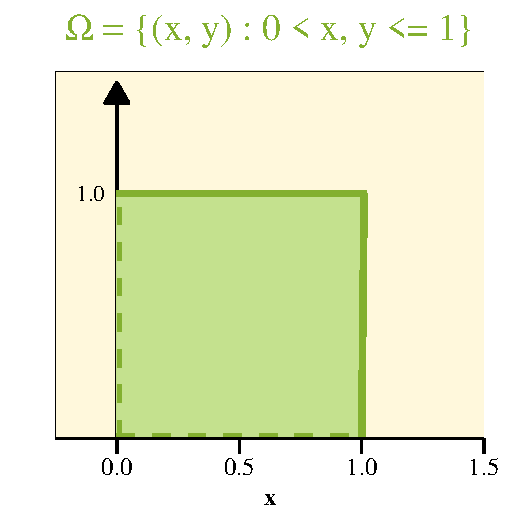
\includegraphics[width=\linewidth]{unit-square.pdf}
  \vspace{-1ex}
\end{minipage}
\hspace*{-1.5em}

\vspace{-0.39\textwidth}

\[
\begin{split}
\begin{gathered}
    \Omega= \{(x, y) : 0 < x, y \leq 1\}\\
    \mathcal{F} = \left\{(x, y) : x \in A,\ 0 < y \leq 1 \,\middle|\, A \in \mathfrak{B} \right\}\\
    P(A)= \lambda(A) \text{ for } A \in \mathcal{F} 
\end{gathered}
\end{split}
\begin{split}
\phantom{aaaaaaaaaaaaaaaaaaaaaaaaaaaaaa}
\end{split}
\]

\textbf{a.} Show that \((\Omega, \mathcal{F}, P)\) is a probability
measure space.

\begin{proofline}
   In order to show that $(\Omega, \mathcal{F}, P)$ is a probability\\[-2pt]
   measure space, we need to show that $\mathcal{F}$ is a $\sigma$-field\\[-2pt]
   on $\Omega$ and that $P$ is a probability measure on $\mathcal{F}$.\\[-5pt]
   
   Each set $A \in \mathcal{F}$ is of the form:
    \[
    A = \{(x, y) \in \Omega : x \in E \} = E \times (0,1] \quad \text{for some Borel set } E \subset (0,1].
    \]
       \\
       

\vspace{-5ex}
\begin{minipage}[t]{0.39\textwidth}
  \vspace{-2ex}
  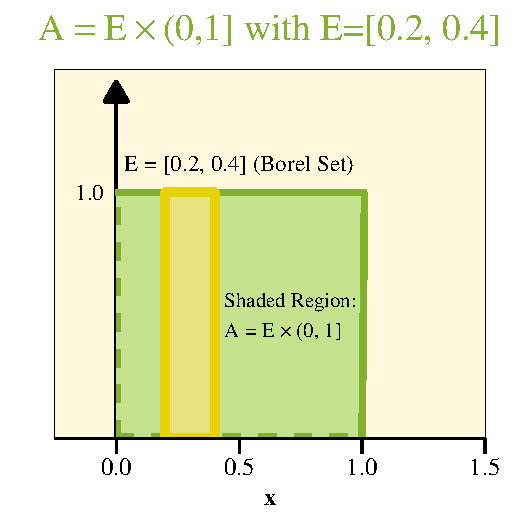
\includegraphics[width=\linewidth]{selected-square.pdf}
  \vspace{-2ex}
\end{minipage}%
\hfill
\begin{minipage}[t]{0.59\textwidth}

    The shaded region to the left represents such a set in $\mathcal{F}$, where
    $E = [0.2, 0.4] \in \mathfrak{B}$. This vertical strip includes every point
    $(x, y) \in \Omega$ such that $x \in E$ and $0 < y \leq 1$.\\[5pt]

    Thus, we can generalize this and say that every set in $\mathcal{F}$ is of the form:
    \[
    A = E \times (0,1] \quad \text{for some } E \in \mathfrak{B}.
    \]

    These are the sets that our probability measure is defined on.\\
\end{minipage}

Our probability measure $P$ is defined on sets $A = E \times (0,1] \in \mathcal{F}$, where $E \in \mathfrak{B}$ is a Borel subset of $(0,1]$. We define $P$ in terms of the Lebesgue measure $\lambda$ on $(0,1]$ as:
\[
P(A) = \lambda(E).
\]

That is, the measure $P$ assigns to each vertical strip $A$ the length of its base set $E$. Intuitively, since the strip $A$ spans the entire height of the unit square from $y = 0$ to $y = 1$, its measure corresponds to the one-dimensional Lebesgue measure of the set of $x$-values it covers.

Formally, this corresponds to defining a product measure:
\[
\lambda_1(E \times (0,1]) = \lambda(E) \cdot \lambda((0,1]) = \lambda(E) \cdot 1 = \lambda(E),
\]
Thus, $\lambda_1$ denotes the product measure formed from the Lebesgue measure on $(0,1]$ applied to the product space $(0,1] \times (0,1]$.

In other words, the measure $P$ on $\mathcal{F}$ is consistent with the one-dimensional Lebesgue measure of the projection of $A$ onto the $x$-axis.

\needspace{6\baselineskip}
\textbf{$\boldsymbol{\mathcal{F}}$ is a $\boldsymbol{\sigma}$-Field on $\boldsymbol{\Omega}$:}
\vspace{-1ex}
\begin{proofline}
    \textbf{$\boldsymbol{\Omega \in \mathcal{F}}$:} 
    $\Omega = (0,1] \times (0,1] = E \times (0,1]$ where $E = (0,1] \in \mathfrak{B}$, so $\Omega \in \mathcal{F}$.
    
    \textbf{$\boldsymbol{\mathcal{F}}$ is closed under complements:} 
    Let $A = E \times (0,1] \in \mathcal{F}$ for some $E \in \mathfrak{B}$. 
    Then
    \vspace{-1ex}
    \[
        \Omega \setminus A = E^c \times (0,1],\ \text{where } E^c \in \mathfrak{B} \Rightarrow A^c \in \mathcal{F}.
    \]
    
    \textbf{$\boldsymbol{\mathcal{F}}$ is closed under countable unions:} 
    Let $A_n = E_n \times (0,1] \in \mathcal{F}$ with $E_n \in \mathfrak{B}$. 
    Then
    \vspace{-3ex}
    \[
        \bigcup_{n=1}^{\infty} A_n = \left( \bigcup_{n=1}^{\infty} E_n \right) \times (0,1],\ \text{which is in } \mathcal{F}.
    \]
  \end{proofline}
  \vspace{1ex}
  \textbf{$\boldsymbol{P}$ is a Probability Measure on $\boldsymbol{\mathcal{F}}$:}
  \vspace{-1ex}
  \begin{proofline}
    \textbf{$\boldsymbol{P(\Omega) = 1}$:}  \quad $P(\Omega) = P((0,1] \times (0,1]) = \lambda((0,1]) = 1.$
    
    \textbf{$\boldsymbol{P}$ is countably additive:} 
    Let $A_n = E_n \times (0,1]$ with $E_n \in \mathfrak{B}$. Then
    \vspace{-1ex}
    \[
        P\left( \bigcup_{n=1}^{\infty} A_n \right) = P\left( \left( \bigcup_{n=1}^{\infty} E_n \right) \times (0,1] \right) = 
        \lambda\left( \bigcup_{n=1}^{\infty} E_n \right) = 
        \sum_{n=1}^{\infty} P(A_n).
    \]
    \end{proofline}

    \hfill\qed
\end{proofline}

\newpage

\textbf{b.} Show for \(A = \{(x, y) : 0 < x \leq 1,\ y = \frac{1}{2}\}\)
that \(P_{\medstar}(A) = 0\) and \(P^{\medstar}(A) = 1\).

\(\Rightarrow\)\textit{Recall:}
\vspace{-0.5ex}

\needspace{8\baselineskip}
\begin{mdframed}
For each subset $A$ of $\Omega$, we define its \textbf{Outer Measure} as the following:
     \vspace{-2ex}
    \[
        P^{\medstar}(A)=\textbf{inf}\sum_n P(A_n) \quad \quad \scalebox{0.8}[0.8]{\textbf{Outer Measure}}
    \]
    where the infimum is taken over all countable collections of sets $A_n \in \mathcal{F}$ such that $A \subseteq \bigcup_{n=1}^{\infty} A_n$.\\[5pt]
    Conversely, we define the \textbf{Inner Measure} as:
    \vspace{-2ex}
    \[
       P_{\medstar}(A)=1- P^{\medstar}(A^c) \quad \quad \scalebox{0.8}[0.8]{\textbf{Inner Measure}}
    \]
\end{mdframed}

\begin{proofline}
    Let $A = \{(x, y) : 0 < x \leq 1,\ y = \frac{1}{2}\}$.\\
    \textbf{Step 1: Show that } $P^{\medstar}(A) = 1$
    \vspace{-1ex}
    \begin{proofline}
        We can cover $A$ with a countable collection of sets $A_n = (0, \frac{1}{n}] \times \left\{\frac{1}{2}\right\}$ for $n = 1, 2, \ldots$.
        Then,
        \[
            P(A_n) = \lambda\left(\left(0, \frac{1}{n}\right]\right) = \frac{1}{n}.
        \]
        Thus,
        \[
            P^{\medstar}(A) = \inf\sum_{n=1}^{\infty} P(A_n) = \inf\sum_{n=1}^{\infty} \frac{1}{n} = 1.
        \]
        
    \end{proofline}
    
    \textbf{Step 2: Show that } $P_{\medstar}(A) = 0$
    \vspace{-2ex}
    \begin{proofline}
       We can cover $A$ with a countable collection of sets $A_n = (0, \frac{1}{n}] \times \left\{\frac{1}{2}\right\}$ for $n = 1, 2, \ldots$.
        Then,
        \[
            P(A_n) = \lambda\left(\left(0, \frac{1}{n}\right]\right) = \frac{1}{n}.
        \]
        Thus,
        \[
            P_{\medstar}(A) = 1 - P^{\medstar}(A^c) = 1 - \inf\sum_{n=1}^{\infty} P(A_n) = 0.
        \]
      \end{proofline}
    \hfill\qed
\end{proofline}

\newpage

\UNsubsection{Non-Measurable Sets} \quad

    There exists sets in $(0,1]$ that lie outside $\mathfrak{B}$.
    
    \textbf{Proof (by Vitali Set):}
    \vspace{-1ex}
    \begin{proofline}
    Begin by defining a custom operator that uses addition modulo 1 in (0,1].
    \[
    x\oplus y = \begin{cases}
        x+y \quad &\text{ if } x+y \leq 1\\
        x+y-1 \quad &\text{ if } x+y > 1
    \end{cases}
    \]

    Let \( \mathcal{L} \) be the class of Borel sets \( A \subset (0,1] \) such that for all \( x \in (0,1] \), the translated set \( A \oplus x \) is Borel and
    \[
    \lambda(A \oplus x) = \lambda(A).
    \]
    
    Then \( \mathcal{L} \) is a \( \lambda \)-system containing the intervals. Since intervals form a \( \pi \)-system generating the Borel \( \sigma \)-field \( \mathcal{B} \), the \( \pi \)-\( \lambda \) theorem implies \( \mathcal{B} \subseteq \mathcal{L} \). Thus, Lebesgue measure \( \lambda \) is translation-invariant.

    Define \( x \sim y \) if \( x = y \oplus r \) for some rational \( r \in (0,1] \). This partitions \( (0,1] \) into disjoint equivalence classes.

    Use the axiom of choice to pick a set \( H \subset (0,1] \) containing exactly one representative from each equivalence class under \( \sim \).

    For each rational \( r \in (0,1] \cap \mathbb{Q} \), define \( H \oplus r = \{ h \oplus r : h \in H \} \). Then
    
    \[
    (0,1] = \bigcup_{r \in \mathbb{Q} \cap (0,1]} \hspace{-1em}H \oplus r,
    \]
    
    is a countable disjoint union.

    If \( H \) were measurable, then so would each \( H \oplus r \) be, and by countable additivity,
    \[
    \lambda((0,1]) = \sum_{r \in \mathbb{Q} \cap (0,1]} \hspace{-1em}\lambda(H \oplus r).
    \]
    But all these sets are translates of \( H \), so each term equals \( \lambda(H) \). The sum is either:
    \begin{itemize}
        \item[$\Rightarrow$] 0, if \( \lambda(H) = 0 \), contradicting \( \lambda((0,1]) = 1 \), \raisebox{-2.5ex}{or}
        \vspace{-2.5ex}
        \item[$\Rightarrow$] \( \infty \), if \( \lambda(H) > 0 \), also a contradiction.
    \end{itemize}
    Thus, no such \( \lambda(H) \) can exist, and we conclude that \( H \notin \mathcal{B} \). As a result, there exist sets \( H \subset (0,1] \) that are not Lebesgue measurable. \hfill \qed
    \end{proofline}

    \newpage